\chapter{Week}
The main focus of this week was research and starting to layout the first presentation. It was assumed that the audience is technology savvy but has no particular background in \ac{AI}. Thus, the presentation had to introduce the whole field and key concepts that enabled the rise of \ac{AI} applications in recent years. The first draft of the presentation was discussed in a meeting and some changes were made to the overall structure, the content and the degree of complexity.The rough structure of the presentation is as follows:
\begin{itemize}
	\item \textbf{Motivation}: To get the viewers interest it was shown that \ac{AI} applications are already part of daily life for everyone. This was achieved by showing that all of the major companies such as Google, Apple, Facebook, Microsoft as well as Tesla, Netflix and Amazon use \ac{AI} in their datacenters and products and allocate huge resources to \ac{AI} research. The importance of \ac{AI} was further enhanced by showing the rapid growth of annually published \ac{AI} papers and startups developing \ac{AI} systems. The trend from 1995 to 2015 resembles almost exponential growth in \ac{AI} research and products.
	\item \textbf{Definition}: As \ac{AI} has become such a buzz word in media a definition of the term was needed and what part of \ac{AI} is actually used in all of the common applications. \ac{ANN} that perform typical computer vision and language processing tasks are all part of \ac{ML}, which is a subset of \ac{AI}. \ac{ML} itself can then be divided into further subsets using roughly three learning methods, supervised learning, unsupervised learning and reinforcement learning. As supervised learning is the most commonly used method, the presentation focused on this method used to train \ac{ANN}. Furthermore, the different parts that comprise a \ac{ANN} are introduced, namely the neuron and how neurons are formed into layers. These layers are then stacked together to form an \ac{ANN}.
	\item \textbf{Key concepts}: An explanation of supervised learning was given with two distinct examples, linear regression and deep learning neural networks to illustrate the idea behind supervised learning: predict a value $y$ given an input $x$ by deploying a function $f(x)$. This function $f(x)$ is acquired by deploying a learning algorithm and usage of a so called training set, consisting of input pairs $x$ and $y$. The concept of inference and training were also explained with an emphasis on inference. Once a network is trained, only inference needs to be run, so this is the crucial part application wise.
	\begin{figure}[!htb]
	\centering
		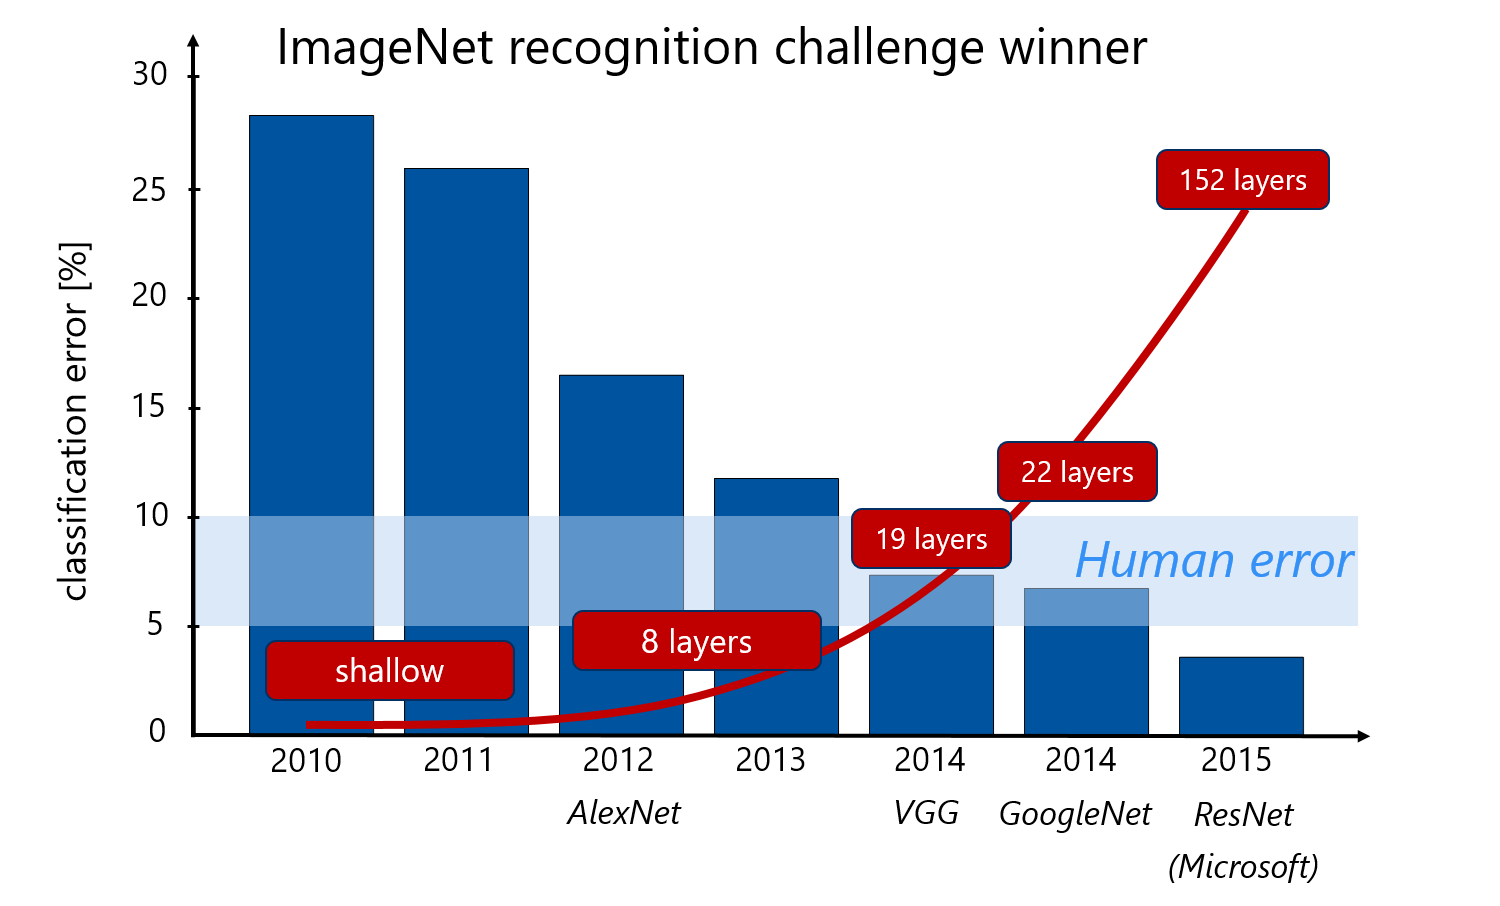
\includegraphics[width=\textwidth]{bilder/ilsvrc.png}
		\caption{ILSVRC winners}
		\label{fig:ilsvrc}
\end{figure}
	\item \textbf{Deep Learning}: Figure~\ref{fig:ilsvrc} shows the winners of the state-of-the-art ImageNet Large Scale Visual Recognition Challenge. It illustrates that the breakthrough in performance came not only from more sophisticated networks, but mainly from stacking different kinds of layers deeply, hence the name. The presentation was ended with the question, what hardware is best suited for \ac{ANN} applications.
\end{itemize}
Alongside preparing the presentation the error preventing the more sophisticated examples was identified as the board crashed while performing tasks related to video analysis (face detection, pose detection, etc.). At first, it was suspected there were some problems with heat management and using the system monitor the temperature of the \ac{FPGA} was investigated during operation. As this seemed to be well within allowed borders specified by the Xilinx data sheet, other causes had to be found.